\documentclass{beamer}

% Solarized Theme
\usecolortheme[light, accent=orange]{solarized}
\beamertemplatenavigationsymbolsempty

% Packages
\usepackage[T1]{fontenc}
\usepackage[utf8]{inputenc}
\usepackage[english]{babel}

\usepackage{multicol}
\usepackage{graphicx}
\usepackage{fontawesome}
\usepackage{xcolor}

\title{\Large{How to make an awesome package in python}}
\author{\textbf{Michalis Panayides}}
\date{}

\begin{document}

    \frame{
        \titlepage
        \centering
        \vspace{-2cm}
        \textbf{PGR-Talks}
    }
    \setbeamertemplate{frametitle}[default][center]

    \begin{frame}
    \frametitle{About me}
    \centering
        
    
\includegraphics[scale=0.1]{Bin/CardiffUniLogo.png}
    
\includegraphics[scale=0.15]{Bin/THISLogo.png}

\end{frame}
    \begin{frame}
    \frametitle{Tools for an awesome python package \\
        {\tiny based on \href{https://antonz.org/python-packaging/}
        {Anton Zhiyanov's blog}}
    }

    \begin{multicols}{2}
        \begin{center}
            {\huge Awesome}
            \only<3>{
                \begin{itemize}
                    \item Documentation
                    \item Testing
                    \item Linters
                    \item Tox
                    \item GitHub actions
                \end{itemize}
            }
        \end{center}
        
        \columnbreak
        {\huge Python Package}
        \only<2,3>{
            \begin{itemize}
                \item Git
                \item GitHub
                \item Python
                \item Flit
            \end{itemize}
        }
    \end{multicols}

\end{frame}

    \begin{frame}
    \frametitle{Version Control with Git}
    \centering
    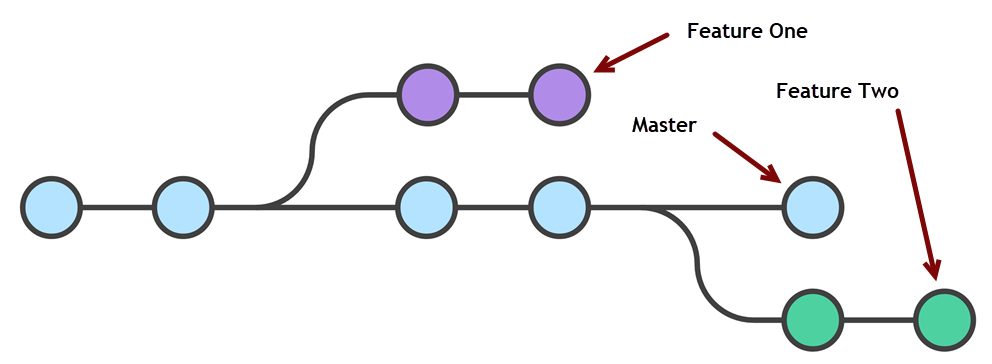
\includegraphics[scale=0.35]{Bin/git.png}
    

    \vspace{0.5cm}
    \pause

    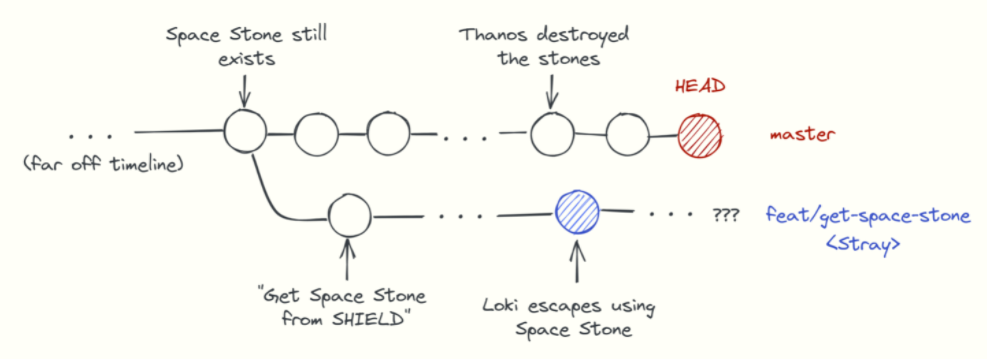
\includegraphics[scale=0.5]{Bin/git_endgame.PNG}

    \href{https://ljvmiranda921.github.io/notebook/2021/06/05/avengers-git/}{Git VS Avengers: Endgame}

\end{frame}


\begin{frame}
    \frametitle{\href{https://git-school.github.io/visualizing-git/}{Git with GitHub}}
    \centering
    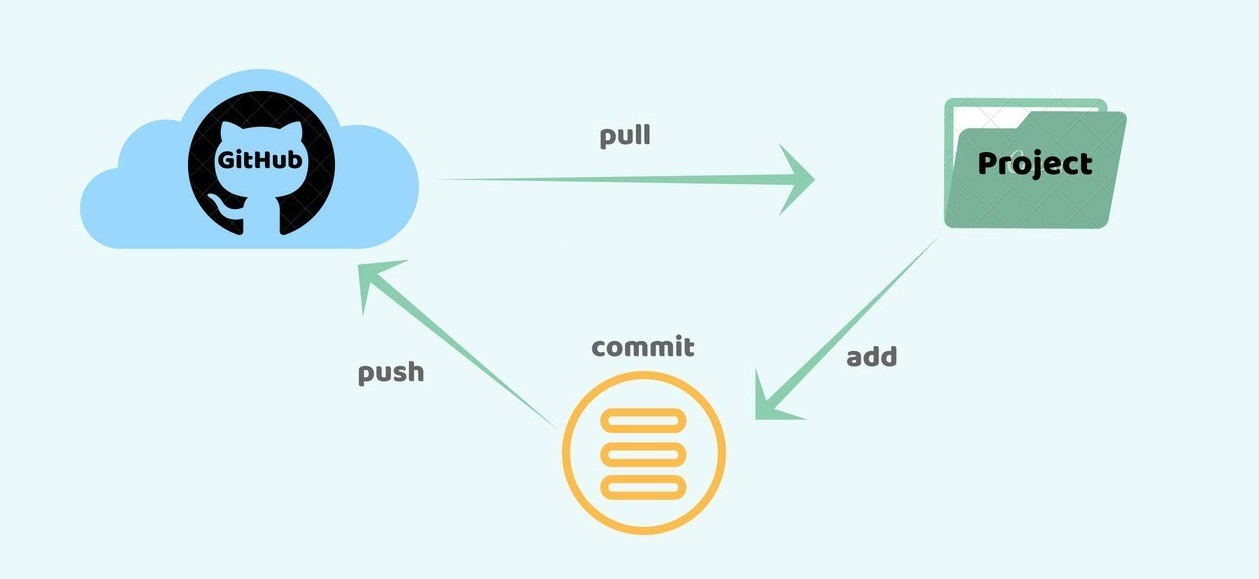
\includegraphics[width=\textwidth, height=0.65\textheight, trim=30 0 50 0, clip]{Bin/github.jpg}

\end{frame}

    \begin{frame}
    \frametitle{Python}
    \centering
    
\includegraphics[scale=0.06]{Bin/python_logo.png}

    \vspace{1cm}
    \pause

    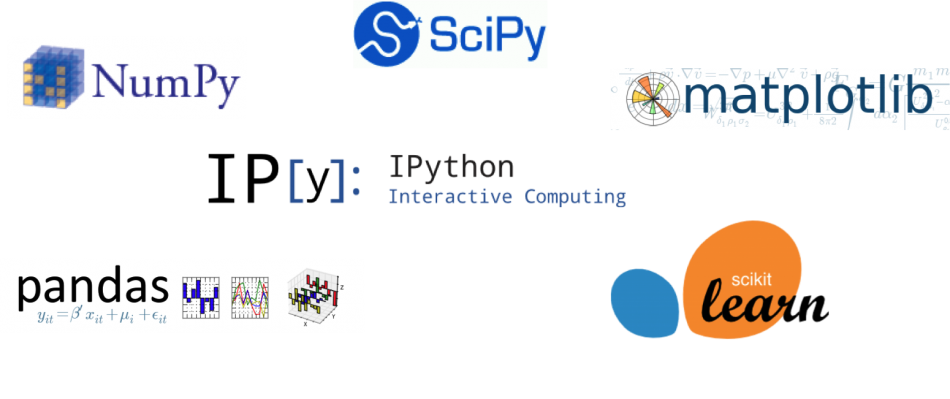
\includegraphics[scale=0.3]{Bin/python_libraries.png}

\end{frame}


\begin{frame}
    \frametitle{Rock-Paper-Scissors}

    \hfuzz = 37pt
    \hspace{3.9cm}
    \vspace{-1cm}
    
\includegraphics[width=.27\textwidth]{Bin/rock-paper-scissors.png}
    \begin{multicols}{3}
        \begin{flushright}
            
\includegraphics[height=0.12\textheight, angle=270]{Bin/rock-paper-scissors.png}
        \end{flushright}
            
        \columnbreak
 
        \begin{equation*}
            \begin{bmatrix}
                0 & & +1 & & -1 \\
                & & & & \\
                -1 & & 0 & & +1 \\
                & & & & \\
                +1 & & -1 & & 0
            \end{bmatrix}
        \end{equation*}

        \columnbreak
        \vfill
    \end{multicols}

\end{frame}



\begin{frame}
    \centering
    
    \begin{multicols}{2}
        {\Large \textbf{\href{https://flit.readthedocs.io/en/latest/upload.html\#using-pypirc}{Flit}}}
        \begin{itemize}
            \item Initialising
            \item Packaging
            \item Publishing
        \end{itemize}

        \columnbreak
        \pause        
        {\Large \textbf{\href{https://pypi.org/}{PyPI} \& \href{https://test.pypi.org/}{TestPyPI}}}
        
\includegraphics[scale=0.1]{Bin/pypi_logo.png}
    \end{multicols}

\end{frame}

    \begin{frame}
    \frametitle{Documentation}

    \begin{itemize}
        \item \textbf{Readme.md}: A markdown file that contains an overview of 
        the project

        \vspace{1cm}

        \item \textbf{Changelog.md}: A file with a log of all the changes ever 
        made to the project

        \vspace{1cm}

        \item \textbf{Docstrings}: A comment in the code that is used to explain 
        a block of code  
    \end{itemize}

\end{frame}
    \begin{frame}
    \frametitle{Testing}
    
    \begin{multicols}{2}
        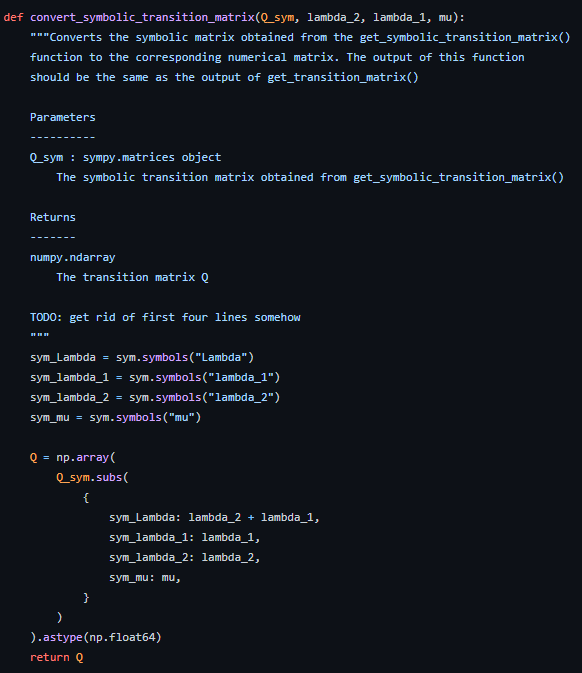
\includegraphics[width=0.48\textwidth]{Bin/ambulance_game_code.PNG}

        \columnbreak

        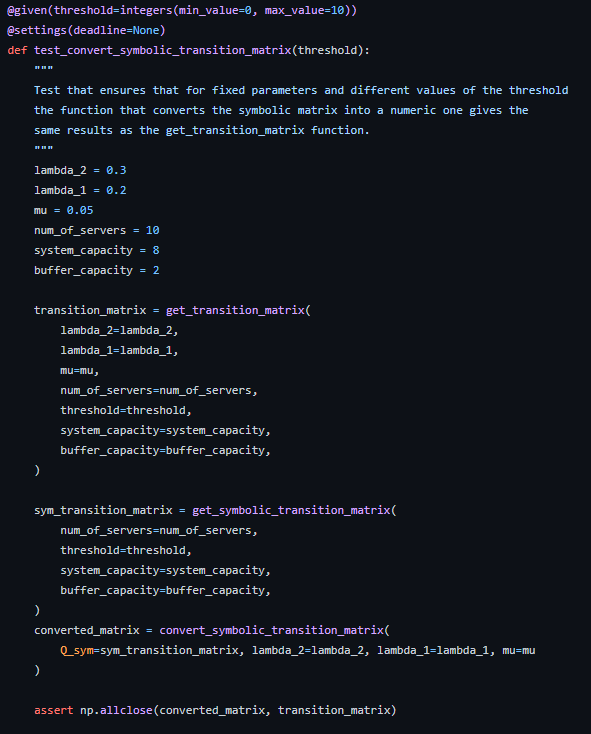
\includegraphics[width=0.48\textwidth]{Bin/ambulance_game_test.PNG}
    \end{multicols}

\end{frame}


\begin{frame}
    \frametitle{Linters}
    \centering

    \textit{Linting} is the automated checking of your source code for 
    programmatic and stylistic errors without running the code
    
    \vspace{1cm}

    Linting tools:
    
    \begin{multicols}{3}
        \begin{itemize}
            \item black
            \item pylint
            \item tox
            \item flake8
            \item mccabe
            \item mypy
        \end{itemize}
    \end{multicols}
\end{frame}


\begin{frame}
    \frametitle{GitHub Actions}

    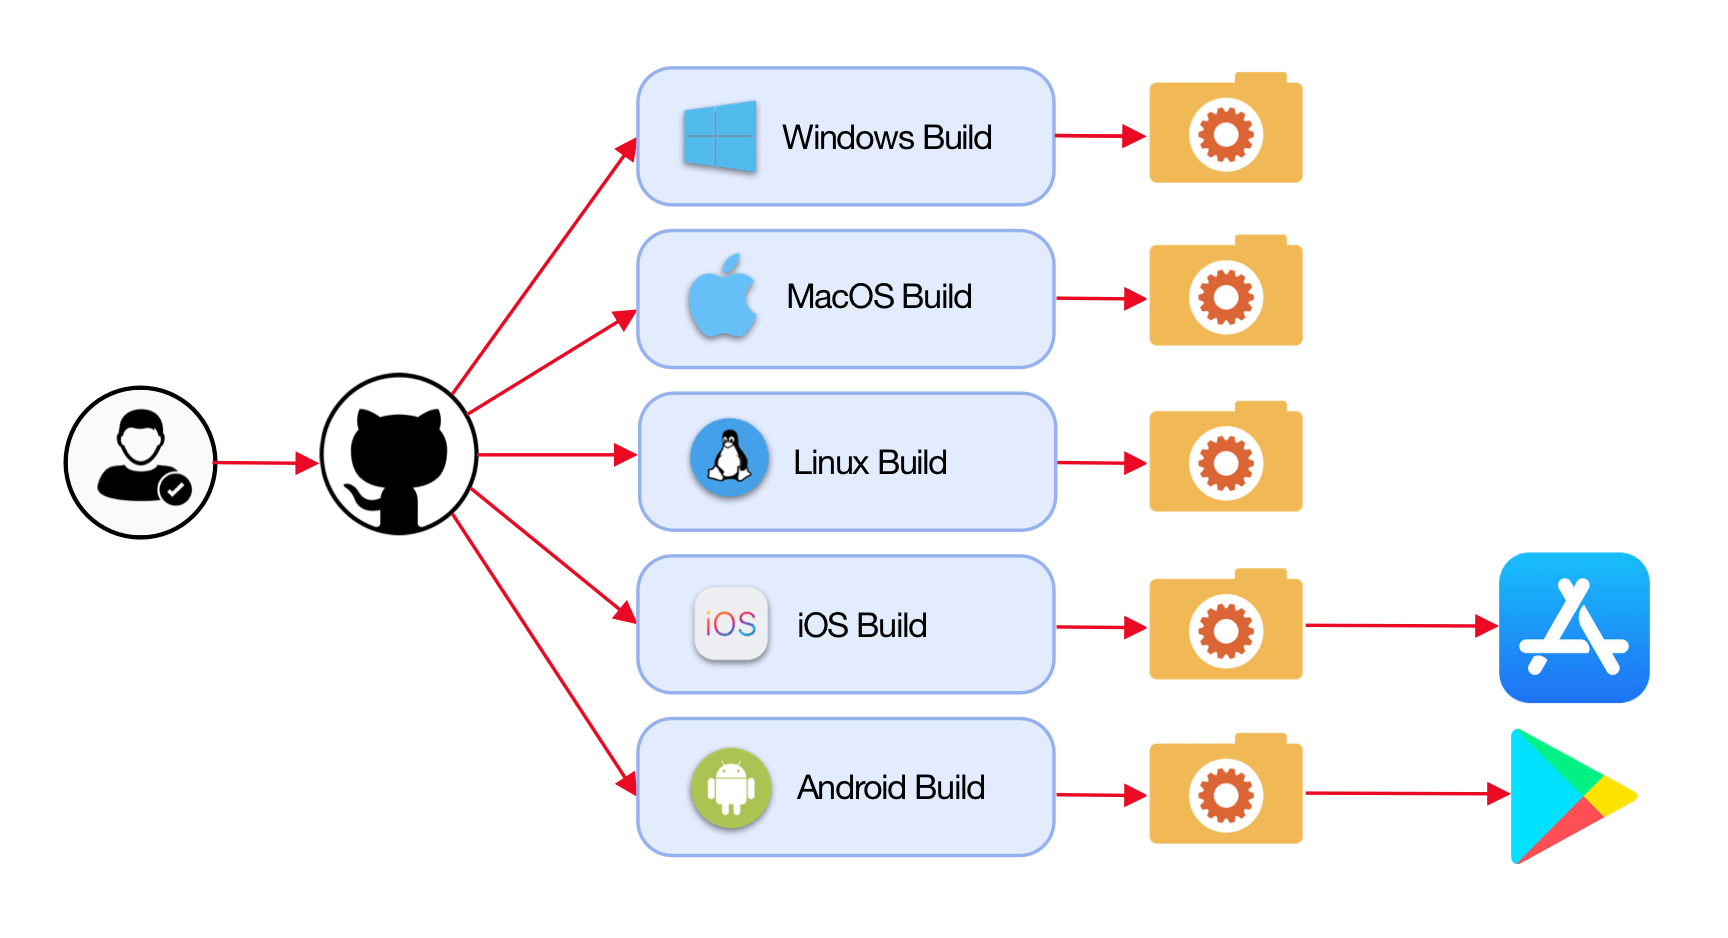
\includegraphics[width=\textwidth]{Bin/github_actions.png}

\end{frame}


    \begin{frame}
    \frametitle{Thank you!}
    \centering

    \vspace{0.8cm}
    \faEnvelope \, \url{PanayidesM@cardiff.ac.uk}

    \vspace{0.8cm}
    \faTwitterSquare \, \url{@Michalis_Pan}

    \vspace{0.8cm}
    \faGithubSquare \, \url{@11michalis11}

\end{frame}


\end{document}